% !TEX program = xelatex
% Build: tectonic -X compile docs/research_overview.tex --outdir docs
\documentclass[aspectratio=169,9pt]{beamer}

\usepackage{fontspec}
\setmainfont{DejaVu Sans}
\setsansfont{DejaVu Sans}
\setmonofont{DejaVu Sans Mono}

\usepackage{graphicx}
\usepackage{booktabs}
\usepackage{array}
\usepackage{colortbl}
\usepackage{amsmath,amssymb}
\usepackage{tikz}
\usetikzlibrary{arrows.meta,positioning,fit,backgrounds}

\setbeamersize{text margin left=0.58cm,text margin right=0.58cm}

\definecolor{Navy}{HTML}{0F2942}
\definecolor{Teal}{HTML}{007A87}
\definecolor{TealLight}{HTML}{E6FFFA}
\definecolor{GreenAccent}{HTML}{2F855A}
\definecolor{GreenBg}{HTML}{F0FFF4}
\definecolor{Coral}{HTML}{C53030}
\definecolor{CoralBg}{HTML}{FFF5F5}
\definecolor{Amber}{HTML}{B7791F}
\definecolor{AmberBg}{HTML}{FFFFF0}
\definecolor{Slate}{HTML}{4A5568}
\definecolor{LightBg}{HTML}{F7FAFC}
\definecolor{BorderGray}{HTML}{CBD5E0}

\usetheme{default}
\usecolortheme{default}
\setbeamertemplate{navigation symbols}{}
\setbeamertemplate{itemize items}{\textcolor{Teal}{$\blacktriangleright$}}
\setbeamercolor{normal text}{fg=black!88}
\setbeamercolor{structure}{fg=Navy}
\setbeamercolor{frametitle}{fg=white,bg=Navy}

\setbeamertemplate{frametitle}{%
  \nointerlineskip%
  \begin{beamercolorbox}[wd=\paperwidth,leftskip=0.58cm,rightskip=0.58cm,sep=0pt]{frametitle}%
    \rule{0pt}{0.50cm}{\normalsize\bfseries\insertframetitle}\par%
    \ifx\insertframesubtitle\@empty\else%
      \vspace{0.04cm}%
      {\scriptsize\normalfont\color{TealLight}\insertframesubtitle}\par%
    \fi%
    \vspace{0.16cm}%
  \end{beamercolorbox}%
  \nointerlineskip%
  {\color{Teal}\hrule height 1.4pt}%
}

\setbeamertemplate{footline}{%
  \leavevmode%
  \hbox{%
    \begin{beamercolorbox}[wd=.82\paperwidth,ht=1.9ex,dp=0.7ex,leftskip=0.58cm]{normal text}%
      \tiny\color{Slate}Hetero-Physical 3:1 Spectral-Reservoir Hybrid LM (0.10B--1.4B) \quad|\quad Open-Science Research Overview (v0.3.0)
    \end{beamercolorbox}%
    \begin{beamercolorbox}[wd=.18\paperwidth,ht=1.9ex,dp=0.7ex,rightskip=0.58cm]{normal text}%
      \hfill\scriptsize\color{Navy}\bfseries\insertframenumber{} / \inserttotalframenumber%
    \end{beamercolorbox}%
  }%
}

\newcommand{\cardbox}[3][LightBg]{%
  \noindent\begin{tikzpicture}
    \node[rectangle,rounded corners=3.5pt,draw=BorderGray,fill=#1,inner sep=4.5pt,text width=\dimexpr #2 - 10pt\relax,align=left,font=\scriptsize] {#3\par};
  \end{tikzpicture}%
}

\newcommand{\badge}[2]{%
  \tikz[baseline=(n.base)]\node[rectangle,rounded corners=2.2pt,fill=#1,draw=none,text=white,font=\tiny\bfseries,minimum height=0pt,minimum width=0pt,text width={},inner xsep=3.8pt,inner ysep=1.5pt,align=center](n){#2};%
}

\newcolumntype{L}[1]{>{\raggedright\arraybackslash}p{#1}}

\begin{document}

% ==============================================================================
% SLIDE 1: TITLE
% ==============================================================================
{
\setbeamertemplate{footline}{}
\begin{frame}[plain]
  \begin{tikzpicture}[remember picture,overlay]
    \fill[Navy] (current page.south west) rectangle (current page.north east);
    \fill[Teal] (current page.south west) rectangle ([yshift=0.30cm]current page.south east);
    \fill[Teal!32!Navy] ([xshift=-3.9cm]current page.north east) -- (current page.north east) -- (current page.south east) -- ([xshift=-1.7cm]current page.south east) -- cycle;
  \end{tikzpicture}
  \vspace{0.60cm}
  \begin{minipage}{0.90\textwidth}
    {\badge{Teal}{Open-Science Scaling Study} \hspace{0.3em} \badge{GreenAccent}{JAX / Flax / Optax / Orbax v0.3.0} \hspace{0.3em} \badge{Amber}{Apache-2.0}}
    \vspace{0.44cm}

    {\color{white}\LARGE\bfseries Do Attention-Light, Analog-Noise-Tolerant\\[0.18em]Language Models Keep Up with Transformers at Scale?}

    \vspace{0.30cm}
    {\color{TealLight}\normalsize Controlled 0.10B--1.4B Architecture, Pilot Findings, XLA Systems Design \& Evaluation Protocol}

    \vspace{0.58cm}
    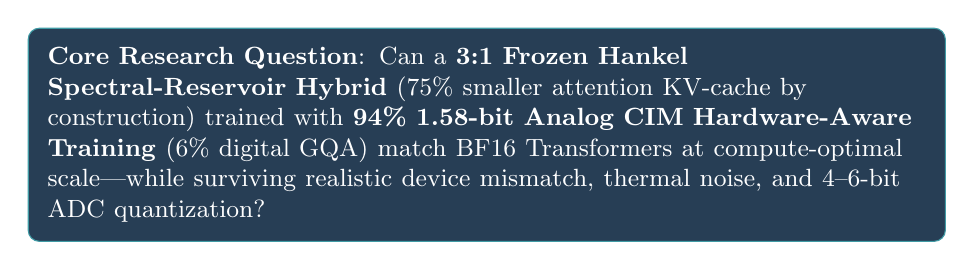
\begin{tikzpicture}
      \node[rounded corners=4pt,fill=white!10!Navy,draw=Teal!75,inner sep=7pt,text width=0.92\textwidth] {
        \color{white!95}\small\raggedright
        \textbf{Core Research Question}: Can a \textbf{3:1 Frozen Hankel Spectral-Reservoir Hybrid} (75\% smaller attention KV-cache by construction) trained with \textbf{94\% 1.58-bit Analog CIM Hardware-Aware Training} (6\% digital GQA) match BF16 Transformers at compute-optimal scale---while surviving realistic device mismatch, thermal noise, and 4--6-bit ADC quantization?\par
      };
    \end{tikzpicture}

    \vspace{0.50cm}
    {\color{white!82}\footnotesize Code \& Tests: \texttt{https://github.com/shukob/hetero-spectral-lm-jax}\\[0.2em]
    \color{white!68}\scriptsize Independent Non-Commercial Open Academic Research \quad|\quad November 2026}
  \end{minipage}
\end{frame}
}

% ==============================================================================
% SLIDE 2: ARCHITECTURES & MATCHED PRESETS
% ==============================================================================
\begin{frame}{Controlled 3-Model Architecture Design \& Parameter-Matched Presets}{Identical 32,768 vocabulary, document order, 2,048 context, $\mu$P scaling, and hybrid Muon+AdamW WSD schedule}
  \vspace{0.02cm}
  \begin{center}
  \resizebox{0.99\textwidth}{!}{%
  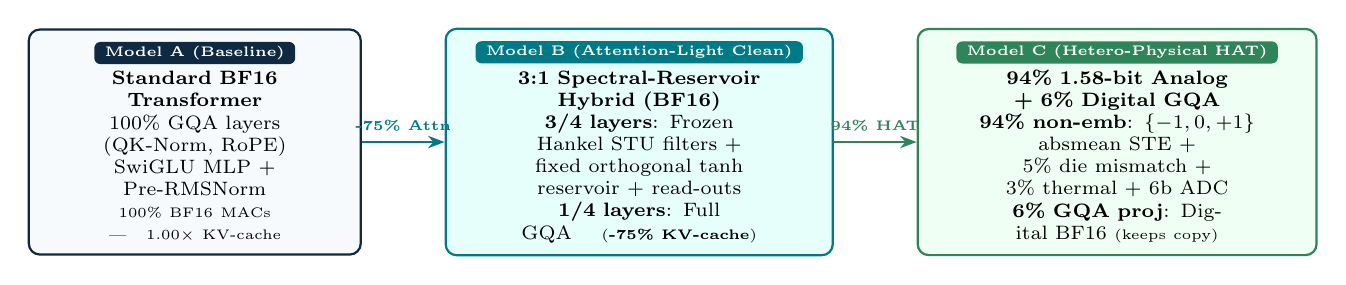
\begin{tikzpicture}[
    box/.style={rectangle,rounded corners=4pt,draw=Navy,thick,align=center,font=\scriptsize,inner sep=4.5pt},
    arr/.style={-{Stealth[length=2.1mm]},thick,Navy}
  ]
    \node[box,fill=LightBg,text width=3.9cm] (ma) {
      \badge{Navy}{Model A (Baseline)}\\[0.28em]
      \textbf{Standard BF16 Transformer}\\
      100\% GQA layers (QK-Norm, RoPE)\\
      SwiGLU MLP + Pre-RMSNorm\\
      {\tiny 100\% BF16 MACs \quad|\quad 1.00$\times$ KV-cache}
    };
    \node[box,draw=Teal,fill=TealLight,right=1.05cm of ma,text width=4.6cm] (mb) {
      \badge{Teal}{Model B (Attention-Light Clean)}\\[0.28em]
      \textbf{3:1 Spectral-Reservoir Hybrid (BF16)}\\
      \textbf{3/4 layers}: Frozen Hankel STU filters +\\
      fixed orthogonal $\tanh$ reservoir + read-outs\\
      \textbf{1/4 layers}: Full GQA \quad {\tiny (\textbf{-75\% KV-cache})}
    };
    \node[box,draw=GreenAccent,fill=GreenBg,right=1.05cm of mb,text width=4.75cm] (mc) {
      \badge{GreenAccent}{Model C (Hetero-Physical HAT)}\\[0.28em]
      \textbf{94\% 1.58-bit Analog + 6\% Digital GQA}\\
      \textbf{94\% non-emb}: $\{-1,0,+1\}$ absmean STE +\\
      5\% die mismatch + 3\% thermal + 6b ADC\\
      \textbf{6\% GQA proj}: Digital BF16 {\tiny (keeps copy)}
    };
    \draw[arr,Teal] (ma.east) -- node[above,font=\tiny\bfseries,color=Teal]{-75\% Attn} (mb.west);
    \draw[arr,GreenAccent] (mb.east) -- node[above,font=\tiny\bfseries,color=GreenAccent]{94\% HAT} (mc.west);
  \end{tikzpicture}%
  }
  \end{center}
  \vspace{0.10cm}
  \begin{columns}[T,totalwidth=\textwidth]
    \begin{column}{0.61\textwidth}
      \textbf{\footnotesize\color{Navy} Exact Parameter Presets (Verified Against Flax Parameter Tree)}\\[0.20em]
      \scriptsize
      \setlength{\tabcolsep}{3.0pt}
      \renewcommand{\arraystretch}{1.22}
      \begin{tabular}{@{}lrrrrr@{}}
        \toprule
        \textbf{Preset} & \textbf{Width / Layers} & \textbf{A (TF)} & \textbf{B/C (Hyb)} & \textbf{Non-Emb $\Delta$} & \textbf{Analog (C)} \\
        \midrule
        \texttt{0.10b} & 768 / 12 (9:3) & 100.68M & 104.37M & +4.88\% & 93.83\% \\
        \texttt{0.26b} & 1024 / 20 (15:5) & 259.04M & 267.95M & +3.95\% & 94.26\% \\
        \texttt{0.65b} & 1536 / 24 (18:6) & 644.95M & 680.93M & +6.05\% & 94.28\% \\
        \rowcolor{TealLight}
        \texttt{1.3b} & 2048 / 28 (21:7) & 1,329.71M & 1,397.62M & +5.38\% & \textbf{94.41\%} \\
        \bottomrule
      \end{tabular}
    \end{column}
    \begin{column}{0.37\textwidth}
      \cardbox[AmberBg]{\linewidth}{
        \textbf{\textcolor{Amber}{Why Passive Fixed Spectral Reservoirs?}}\\[0.22em]
        $\bullet$ \textbf{BIBO Passive Stability}: Fixed Hankel convolution filters cannot exponentially amplify multiplicative analog noise (unlike recurrent SSMs).\\[0.22em]
        $\bullet$ \textbf{Minimal Digital Island}: Keeping only sparse GQA projections ($\sim$6\%) digital preserves exact long-range copying while offloading 94\% of weights to multiplier-free 1.58-bit CIM.
      }
    \end{column}
  \end{columns}
\end{frame}

% ==============================================================================
% SLIDE 3: 6-AXIS ADVANTAGE MATRIX
% ==============================================================================
\begin{frame}{Where Are the Advantages? 6-Axis Architectural Comparison Matrix}{Raw short-context GPU tok/s alone hides KV memory, weight/multiplier savings, and analog-noise resilience}
  \vspace{0.02cm}
  \scriptsize
  \setlength{\tabcolsep}{3.5pt}
  \renewcommand{\arraystretch}{1.19}
  \begin{tabular}{@{}>{\bfseries}L{2.30cm}L{2.80cm}L{2.95cm}L{3.25cm}L{2.30cm}@{}}
    \toprule
    \textbf{Axis} & \textbf{Model A: BF16 TF} & \textbf{Model B: 3:1 Res (BF16)} & \textbf{Model C: 94\% Analog HAT} & \textbf{Ref: DeltaNet HAT} \\
    \midrule
    1. Pilot Val CE\newline{\tiny (26.2M tok, lower=better)} &
      0.10B: \texttt{3.769} (PPL 43.4)\newline 0.26B: \texttt{3.724} (PPL 41.4) &
      \textbf{\textcolor{Teal}{0.10B: \texttt{3.712} (PPL 41.0)}}\newline \textbf{\textcolor{Teal}{0.26B: \texttt{3.692} (PPL 40.1)}} &
      0.10B: \texttt{3.977} (6b CIM active)\newline 0.26B: \texttt{3.899} {\tiny (gap shrinks)} &
      0.10B: \texttt{5.159}\newline \textcolor{Coral}{\textbf{Diverges (PPL 174)}} \\
    \rowcolor{LightBg}
    2. Copy Recall $\ge$64\newline{\tiny (n=4,137 real positions)} &
      \texttt{79.2\%} (Clean)\newline {\tiny Drops to \texttt{46.3\%} w/ HAT} &
      \textbf{\textcolor{Teal}{\texttt{81.0\%} (0.10B)}}\newline {\tiny \texttt{79.9\%} (0.26B); -75\% Attn} &
      \textbf{\textcolor{GreenAccent}{\texttt{68.3\%} (0.10B) / \texttt{69.6\%} (0.26B)}}\newline {\tiny \textbf{+22.0 pt} over TF HAT} &
      \texttt{33.4\%}\newline \textcolor{Coral}{\textbf{Collapses}} \\
    3. 64K KV-Cache\newline{\tiny (Inference VRAM / conc.)} &
      0.10B: \texttt{768 MiB}\newline 0.26B: \texttt{1,280 MiB} &
      \textbf{\textcolor{Teal}{0.10B: \texttt{192 MiB} (-75\%)}}\newline \textbf{\textcolor{Teal}{0.26B: \texttt{320 MiB} (-75\%)}} &
      \textbf{\textcolor{GreenAccent}{0.10B: \texttt{192 MiB} (-75\%)}}\newline \textbf{\textcolor{GreenAccent}{0.26B: \texttt{320 MiB} (-75\%)}} &
      \texttt{193 MiB} (-75\%)\newline {\tiny (Unusable under noise)} \\
    \rowcolor{LightBg}
    4. Weights \& MACs\newline{\tiny (Non-embedding)} &
      16.0 bit/param\newline 100\% BF16 multipliers &
      16.0 bit/param\newline 3/4 mixers frozen passive &
      \textbf{\textcolor{GreenAccent}{$\sim$2.44 bit/param (6.5$\times$ lighter)}}\newline \textbf{\textcolor{GreenAccent}{94\% multiplier-free}} $\{-1,0,+1\}$ &
      Multiplier-free possible,\newline fails under CIM noise \\
    5. 1.58b+CIM Eval\newline{\tiny (5\% dev, 3\% therm, 6b/4b)} &
      Clean deploy: \texttt{6.37} \textcolor{Coral}{(fail)}\newline TF HAT: \texttt{4.36} (PPL 78.6) &
      Clean deploy: \texttt{5.38}--\texttt{5.49}\newline \textcolor{Coral}{(unadapted collapse)} &
      \textbf{\textcolor{GreenAccent}{0.10B \texttt{4.09} $\rightarrow$ 0.26B \texttt{4.02}}}\newline {\tiny 4b harsh: \texttt{4.06}; chip $\Delta \le$ \texttt{0.002}} &
      \texttt{5.26} (PPL 193)\newline \textcolor{Coral}{\textbf{Fails}} \\
    \rowcolor{LightBg}
    6. Opt. GPU Train\newline{\tiny (L=2048; JAX \& PyTorch)} &
      \textbf{\textcolor{Navy}{1.00$\times$ baseline}}\newline {\tiny Fastest on BF16 GPU} &
      JAX: \textbf{\texttt{0.82}--\texttt{0.84}$\times$}\newline PT A6000: \textbf{\texttt{0.66}--\texttt{0.97}$\times$} &
      JAX: \textbf{\texttt{0.80}--\texttt{0.81}$\times$}\newline PT A6000: \textbf{\texttt{0.59}--\texttt{0.74}$\times$} {\tiny (2.7$\times$ opt)} &
      --- {\tiny (Unoptimized)} \\
    \midrule
    \rowcolor{AmberBg}
    \textcolor{Amber}{Open Scale Risk}\newline{\tiny (Honest Scope)} &
      Mature baseline &
      Does B track A at 2B--100B tok? &
      Equal-scope unseen-chip + hardware tok/J &
      Excluded from scaling \\
    \bottomrule
  \end{tabular}
\end{frame}

% ==============================================================================
% SLIDE 4: PRELIMINARY PILOT EVIDENCE
% ==============================================================================
\begin{frame}{Preliminary Pilot Evidence (0.10B--0.26B, 26.2M Tokens, 1 Seed)}{Early signals on 2$\times$ RTX A6000 BF16 (seq\_len=2048) motivating compute-optimal TPU scaling}
  \vspace{-0.06cm}
  \begin{center}
    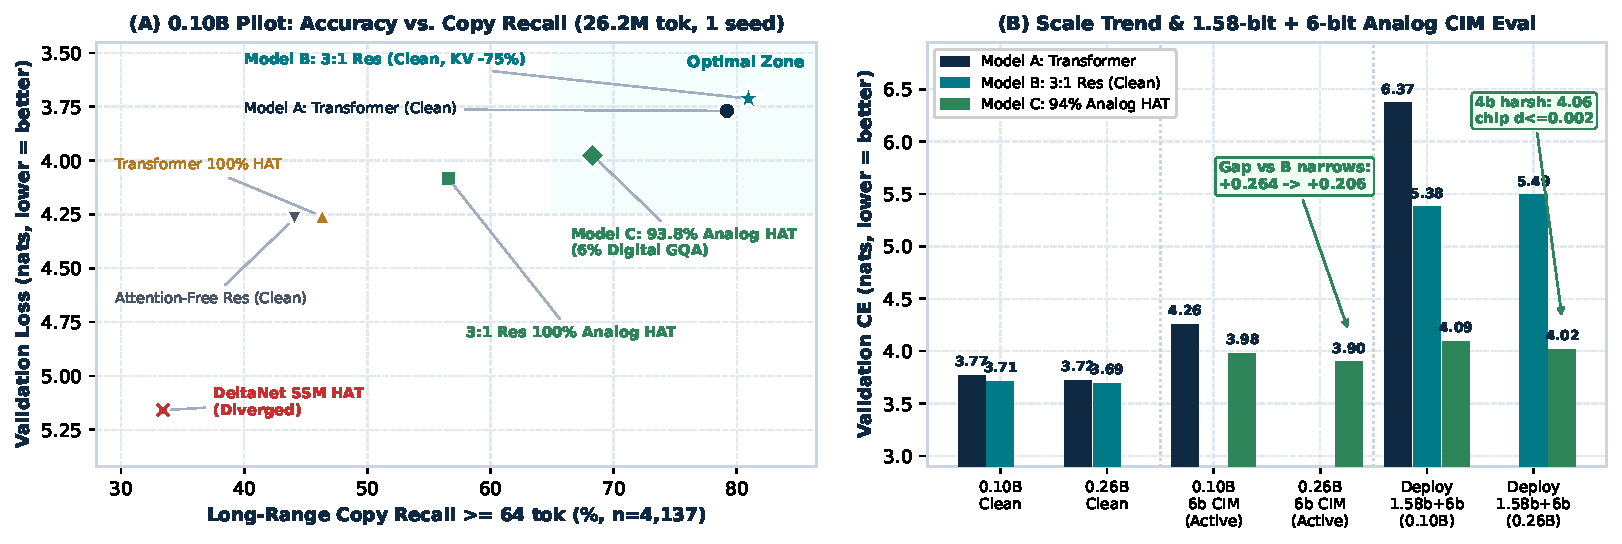
\includegraphics[width=0.98\textwidth,height=0.49\textheight,keepaspectratio]{figs/fig1_pilot_tradeoff.pdf}
  \end{center}
  \vspace{-0.14cm}
  \begin{columns}[T,totalwidth=\textwidth]
    \begin{column}{0.323\textwidth}
      \cardbox[TealLight]{\linewidth}{\textbf{\textcolor{Teal}{1. Attention-Light Parity + Copy}}\\[0.15em]Model B cuts KV-cache by 75\% yet hits \textbf{3.712 vs.\ 3.769} nats (0.10B), \textbf{3.692 vs.\ 3.724} (0.26B), and \textbf{81.0\% vs.\ 79.2\%} copy recall (0-Attn drops to 44.1\%).}
    \end{column}
    \begin{column}{0.323\textwidth}
      \cardbox[GreenBg]{\linewidth}{\textbf{\textcolor{GreenAccent}{2. Passive Reservoir Wins HAT}}\\[0.15em]Under 1.58b + 6-bit analog CIM, Model C beats TF HAT by \textbf{-0.283 nats} and \textbf{+22.0 pt} copy recall, while recurrent DeltaNet HAT diverges (\textbf{5.159 nats / PPL 174}).}
    \end{column}
    \begin{column}{0.323\textwidth}
      \cardbox[AmberBg]{\linewidth}{\textbf{\textcolor{Amber}{3. Honest Scope Controls}}\\[0.15em]Pilot runs are 1-seed at 26.2M tok; 0.26B clean-B vs.\ HAT-C eval probes differed in GQA scope (170 vs.\ 150 modules). Equal-scope unseen-chip \& calibrated controls run at TPU scale.}
    \end{column}
  \end{columns}
\end{frame}

% ==============================================================================
% SLIDE 5: JAX/XLA v0.3.0 & PYTORCH SYSTEMS ENGINEERING
% ==============================================================================
\begin{frame}{Systems Engineering (v0.3.0): Closing the GPU/XLA Throughput Gap}{Exact zero-approximation optimizations (0.00e+00 / $<$1e-5 parity) bring B/C to 0.80--0.84$\times$ TF in JAX}
  \vspace{-0.06cm}
  \begin{center}
    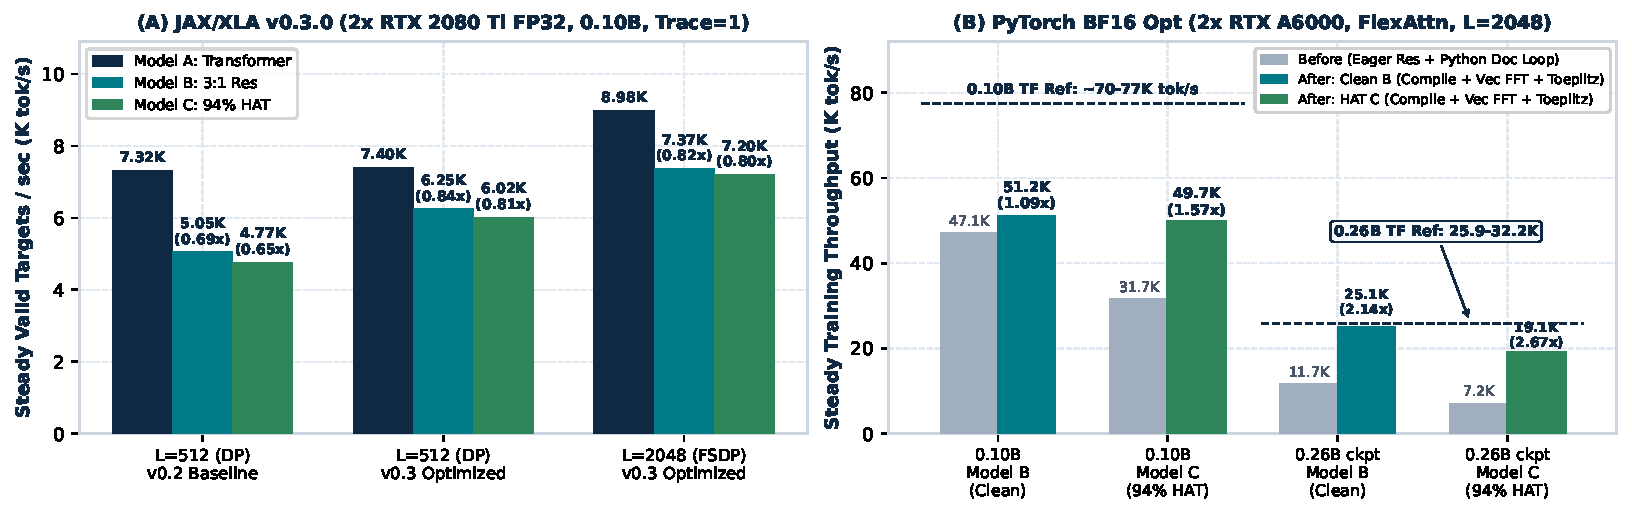
\includegraphics[width=0.98\textwidth,height=0.49\textheight,keepaspectratio]{figs/fig2_systems_throughput.pdf}
  \end{center}
  \vspace{-0.14cm}
  \begin{columns}[T,totalwidth=\textwidth]
    \begin{column}{0.323\textwidth}
      \cardbox[TealLight]{\linewidth}{\textbf{\textcolor{Teal}{Dyadic Static Packing (JAX)}}\\[0.15em]Hall's-theorem buckets \texttt{(256x16, 512x4, 1024x2, 2048x1)} cut L=2048 FFT work \textbf{12$\times\to$5$\times$} and \texttt{n\_fft=4096} slots \textbf{8$\times$}, with \textbf{0.00e+00 leak}, \textbf{1 XLA trace}, and zero collectives.}
    \end{column}
    \begin{column}{0.323\textwidth}
      \cardbox[GreenBg]{\linewidth}{\textbf{\textcolor{GreenAccent}{Precomp FFT + Toeplitz GEMM}}\\[0.15em]Host-cached Hankel spectra eliminate per-layer \texttt{rfft($\phi$)}. Short-bucket ($S\le 256$) reservoir convs run as exact causal Toeplitz GEMMs (\textbf{$<$1e-5} parity; \textbf{2.1$\times$} GPU speedup, MXU-native on TPU).}
    \end{column}
    \begin{column}{0.323\textwidth}
      \cardbox[LightBg]{\linewidth}{\textbf{\textcolor{Navy}{Production TPU / Multi-GPU Ready}}\\[0.15em]\texttt{jax.nn.dot\_product\_attention}, full $\mu$P, tracked-step WSD Muon+AdamW, 1D FSDP (16 GiB HBM compatible), and async \texttt{gs://}-safe Orbax with \textbf{bitwise 0.0} state restore.}
    \end{column}
  \end{columns}
\end{frame}

% ==============================================================================
% SLIDE 6: FALSIFIABLE HYPOTHESES & SCALING PLAN
% ==============================================================================
\begin{frame}{Falsifiable Hypotheses (H1--H3) \& Compute-Optimal Scaling Plan}{Testing whether early pilot trends survive compute-optimal ($\sim$20 tok/param) and overtrained (100B) horizons}
  \vspace{0.04cm}
  \begin{columns}[T,totalwidth=\textwidth]
    \begin{column}{0.46\textwidth}
      \cardbox[TealLight]{\linewidth}{
        \badge{Teal}{H1: Attention-Light Scaling Parity}\\[0.22em]
        At equal scale and tokens up to \textbf{1.3B--1.4B}, Model B stays within \textbf{$\le$0.03 nats/token} of Model A in held-out CE (paired document-bootstrap CIs + multi-seed spread).
      }\\[0.28em]
      \cardbox[GreenBg]{\linewidth}{
        \badge{GreenAccent}{H2: Analog HAT Convergence \& Robustness}\\[0.22em]
        Model C's loss penalty vs.\ B narrows with scale under both nominal 6-bit simulation and ternary-only eval; under \textbf{equal-scope unseen-chip} eval (6/4/3-bit ADC, incl.\ ADC-calibrated clean B), C beats clean B.
      }\\[0.28em]
      \cardbox[LightBg]{\linewidth}{
        \badge{Navy}{H3: Sparse-GQA Copy Mechanism}\\[0.22em]
        Model B and C retain \textbf{$\ge$60\%} accuracy on repeated token pairs separated by $\ge$64 tokens, and masking the earlier occurrence degrades accuracy in both 64--255 and $\ge$256 ranges.
      }
    \end{column}
    \begin{column}{0.52\textwidth}
      \textbf{\footnotesize\color{Navy} Staged Scaling Budget ($\sim 1.8\times 10^{21}$ Total Model FLOPs)}\\[0.20em]
      \scriptsize
      \setlength{\tabcolsep}{2.6pt}
      \renewcommand{\arraystretch}{1.20}
      \begin{tabular}{@{}L{1.45cm}L{3.32cm}rr@{}}
        \toprule
        \textbf{Phase} & \textbf{Matched A / B / C Runs} & \textbf{Tok/Run} & \textbf{FLOPs} \\
        \midrule
        Days 1--10 & Multi-host BF16 L=2048 bring-up & --- & Bring-up \\
        \rowcolor{TealLight}
        Days 11--30 & 0.10B (3s), 0.26B (2s), 0.65B (1s) & 2/5/13B & $2.1\!\times\!10^{20}$ \\
        Days 31--90 & 0.65B (2nd s), 1.3B--1.4B (1s) & 13/27B & $8.3\!\times\!10^{20}$ \\
        Days 31--90 & Overtrained 0.65B pair (A vs.\ B) & 100B & $7.9\!\times\!10^{20}$ \\
        \bottomrule
      \end{tabular}
      \vspace{0.26em}
      \cardbox[AmberBg]{\linewidth}{
        \textbf{\textcolor{Amber}{Data, Fallback Priority \& Open Release}}:\\[0.14em]
        $\bullet$ \textbf{Public Redistributable Corpora Only}: Common Pile, JP Wikipedia (CC BY-SA), permissive code, FineWeb-Edu \& FineWeb-2 JA (ODC-By); staged 15B $\to$ 100B dedup tokens.\\[0.12em]
        $\bullet$ \textbf{Fallback Priority}: Cut 100B pair first, then 1.3B--1.4B, preserving the full 0.10B--0.65B A/B/C comparison.\\[0.12em]
        $\bullet$ \textbf{Negative Results Included}: Code, simulator, logs, checkpoints, and preprint released openly regardless of H1--H3 outcome.
      }
    \end{column}
  \end{columns}
\end{frame}

% ==============================================================================
% SLIDE 7: CONCLUSIONS, HONEST LIMITATIONS & OPEN ARTIFACTS
% ==============================================================================
\begin{frame}{Current Conclusions, Honest Limitations \& Reproducible Artifacts}{Clear separation between verified findings today and hypotheses awaiting compute-optimal scale}
  \vspace{0.04cm}
  \begin{columns}[T,totalwidth=\textwidth]
    \begin{column}{0.51\textwidth}
      \cardbox[GreenBg]{\linewidth}{
        \badge{GreenAccent}{Established Today (Verified)}\\[0.22em]
        $\bullet$ \textbf{Structural Efficiency}: 3:1 Spectral-Reservoir cuts attention KV-cache by \textbf{75\%}; 94\% 1.58-bit HAT cuts non-embedding weights \textbf{6.5$\times$} ($\sim$2.44 b/p) and removes 94\% of multipliers.\\[0.16em]
        $\bullet$ \textbf{Pilot Viability}: Clean B matches/beats A at 26.2M tok while keeping 81.0\% copy recall; HAT C beats TF HAT by \textbf{+22 pt} copy and avoids DeltaNet recurrence divergence.\\[0.16em]
        $\bullet$ \textbf{XLA / GPU Systems}: Exact optimizations (dyadic packing, precomp FFTs, Toeplitz GEMM, coarse compile) recover \textbf{0.80--0.84$\times$} TF in JAX and \textbf{1.6--2.7$\times$} speedups on A6000 BF16.
      }\\[0.28em]
      \cardbox[CoralBg]{\linewidth}{
        \badge{Coral}{Not Yet Proven (Honest Limitations)}\\[0.22em]
        $\bullet$ \textbf{Horizon}: Pilot runs are 26.2M tok ($n$=1 seed); whether B stays within 0.03 nats of A at 20 tok/param and 100B tok is \textbf{unknown}.\\[0.16em]
        $\bullet$ \textbf{Hardware Speedups}: 1.58-bit/analog inference speed \& tok/J gains require dedicated kernels/FPGA/CIM silicon, not BF16 GPU training.\\[0.16em]
        $\bullet$ \textbf{Equal-Scope Eval}: Unseen-chip 6/4/3-bit sweeps with identical GQA scope and ADC-calibrated clean B controls remain to be run at scale.
      }
    \end{column}
    \begin{column}{0.47\textwidth}
      \cardbox[LightBg]{\linewidth}{
        \badge{Navy}{Public Repository (v0.3.0, Apache-2.0)}\\[0.22em]
        \texttt{https://github.com/shukob/hetero-spectral-lm-jax}\\[0.35em]
        \textbf{Automated Verification Suite (8 passed on GPU \& CPU)}:\\[0.14em]
        $\checkmark$ \textbf{$<$1e-6 FP32 Parity}: Checked-in PyTorch reference fixture (Hankel, contracted FFT, 1.58b STE, 6b ADC, 5-step Muon NS).\\[0.12em]
        $\checkmark$ \textbf{0.00e+00 Cross-Doc Leakage}: Perturbing Doc 0 yields exact 0.0 logit diff on Doc 1 + strict API guards.\\[0.12em]
        $\checkmark$ \textbf{1 XLA JIT Trace}: Variable doc layouts in FP32 \& BF16.\\[0.12em]
        $\checkmark$ \textbf{Dyadic L=2048 Stress}: Zero overflow across 200 seeds ($\le$5$\times$ pad) + $<$1e-5 Toeplitz vs.\ FFT parity.\\[0.12em]
        $\checkmark$ \textbf{Async GCS Orbax Resume}: Bitwise \textbf{0.0} param/opt/RNG restore + $<$1e-5 continuation parity.\\[0.38em]
        \textbf{Quickstart}:\\
        {\tiny\ttfamily
        pip install -e ".[dev]" \&\& pytest -v\\
        python -m hetero\_spectral\_lm.train --preset 0.10b \textbackslash\\
        \ \ --arch-mode hybrid\_reservoir --analog-hat --fsdp \textbackslash\\
        \ \ --seq-len 2048 --batch-size 2 --steps 6\par
        }
      }
    \end{column}
  \end{columns}
\end{frame}

\end{document}
